\usetikzlibrary{fit}
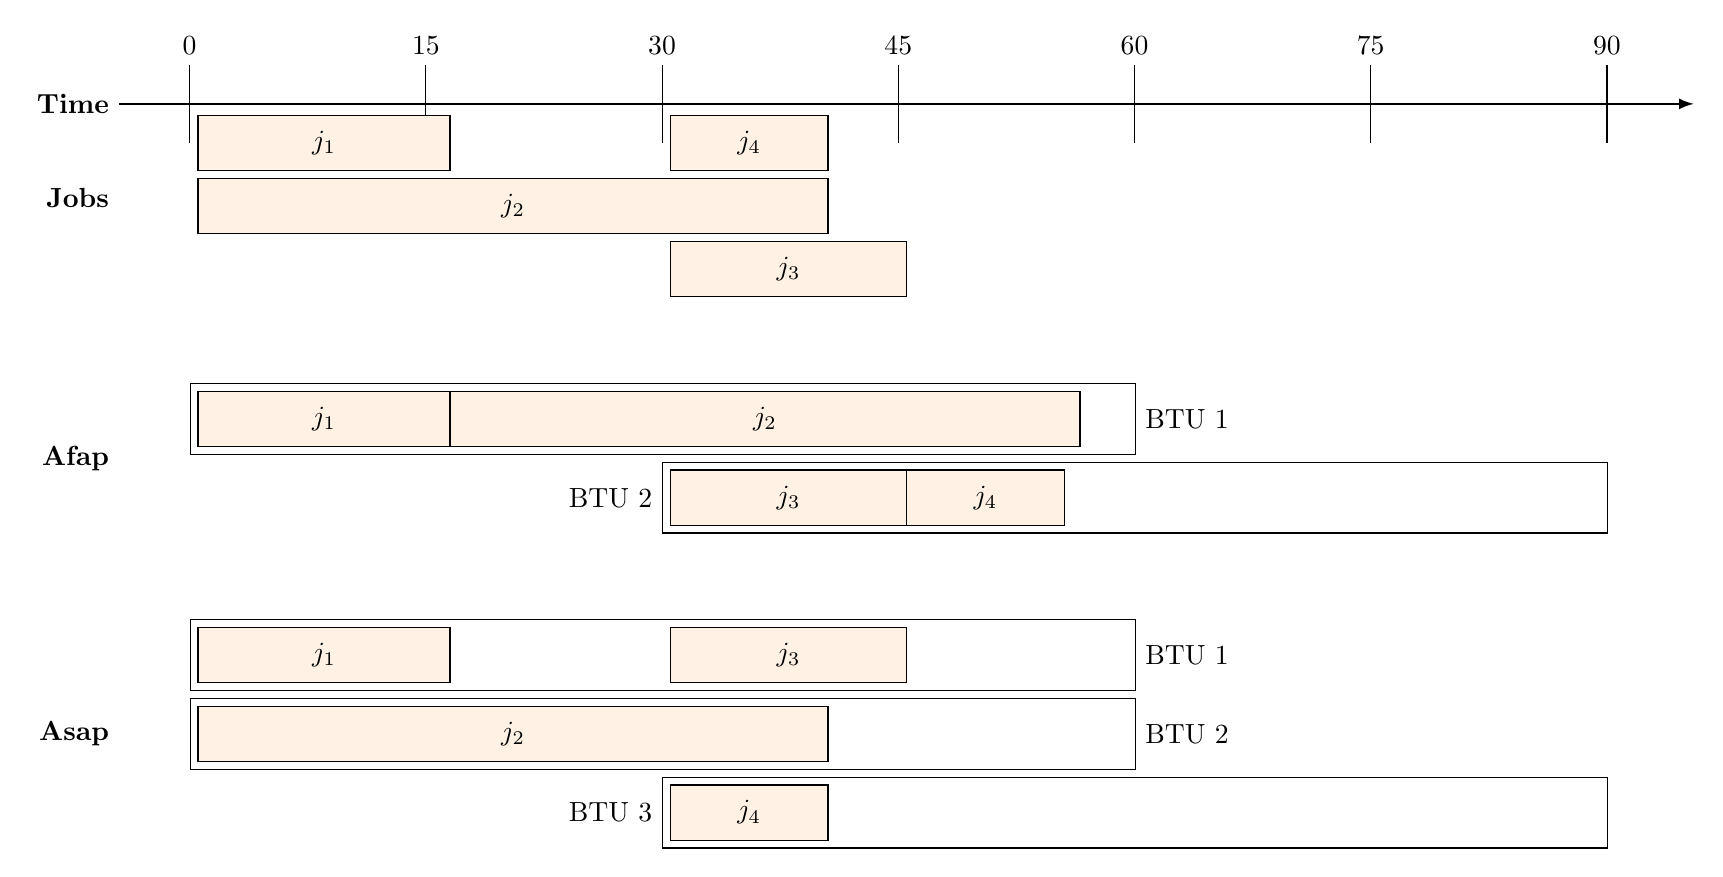
\begin{tikzpicture}[x=2mm,
job/.style={%
anchor=west,
fill=orange!10,
minimum height=7mm,
draw
},
btu/.style={%
anchor=west,
draw,
minimum height=9mm,
minimum width=120mm,
},
strat/.style={%
font=\bfseries,
anchor=east,
align=right,
},
]
%% Timeline
\node[strat]at(-5,0){Time};
\node[strat]at(-5,-1.2){Jobs};
\draw[-{latex},thick] (-5,0)--(95,0);
\foreach \x in {0,15,...,90}{%
\draw (\x-0.5,-0.5)--(\x-0.5,0.5) node[anchor=south]{\x};
}
%% Jobs
\node[job,minimum width=32mm]at(0,-0.5){$j_1$};
\node[job,minimum width=80mm]at(0,-1.3){$j_2$};
\node[job,minimum width=30mm]at(30,-2.1){$j_3$};
\node[job,minimum width=20mm]at(30,-0.5){$j_4$};
%\begin{scope}[shift={(0,2)}]
%% 1vm4all
%\node[strat]at(-5,0){1 VM for all};
%\node[job,minimum width=20mm]at(0,0){$j_1$};
%\node[job,minimum width=80mm]at(10,0){$j_2$};
%\node[job,minimum width=30mm]at(50,0){$j_3$};
%\node[job,minimum width=24mm]at(65,0){$j_4$};
%\node[btu,label={north:BTU 1}]at(-0.5,0){};
%\node[btu,label={north:BTU 2}]at(59.5,0){};
%\end{scope}
%\begin{scope}[shift={(0,4)}]
%% 1VM/job
%\node[strat]at(-5,1.5){1 VM per Job};
%\node[job,minimum width=20mm]at(0,3){$j_1$};
%\node[job,minimum width=80mm]at(0,2){$j_2$};
%\node[job,minimum width=30mm]at(30,1){$j_3$};
%\node[job,minimum width=24mm]at(30,0){$j_4$};
%\node[btu,label={east:BTU 1}]at(-0.5,3){};
%\node[btu,label={east:BTU 2}]at(-0.5,2){};
%\node[btu,label={west:BTU 3}]at(29.5,1){};
%\node[btu,label={west:BTU 4}]at(29.5,0){};
%\end{scope}
\begin{scope}[shift={(0,-4)}]
%% Afap
\node[strat]at(-5,-.5)(f1){Afap};
\node[job,minimum width=32mm]at(0,0){$j_1$};
\node[job,minimum width=80mm]at(16,0){$j_2$};
\node[job,minimum width=30mm]at(30,-1){$j_3$};
\node[job,minimum width=20mm]at(45,-1){$j_4$};
\node[btu,label={east:BTU 1}]at(-0.5,-0)(f2){};
\node[btu,label={west:BTU 2}]at(29.5,-1)(f3){};
\end{scope}
\begin{scope}[shift={(0,-7)}]
%% Asap
\node[strat]at(-5,-1){Asap};
\node[job,minimum width=32mm]at(0,0){$j_1$};
\node[job,minimum width=80mm]at(0,-1){$j_2$};
\node[job,minimum width=30mm]at(30,0){$j_3$};
\node[job,minimum width=20mm]at(30,-2){$j_4$};
\node[btu,label={east:BTU 1}]at(-0.5,0){};
\node[btu,label={west:BTU 3}]at(29.5,-2){};
\node[btu,label={east:BTU 2}]at(-0.5,-1){};
\end{scope}
\end{tikzpicture}
